\chapter{External Services - Components Level - Logical View}
\label{AppendixC2}

This Appendix presents the logical view, component level, of all backend containers related to the \gls{PoC}s developed.

The \textit{AMQP API} is the one represented as \textit{Sensae API for External Services} in most logical diagrams.

\begin{figure}[H]
   \centering
   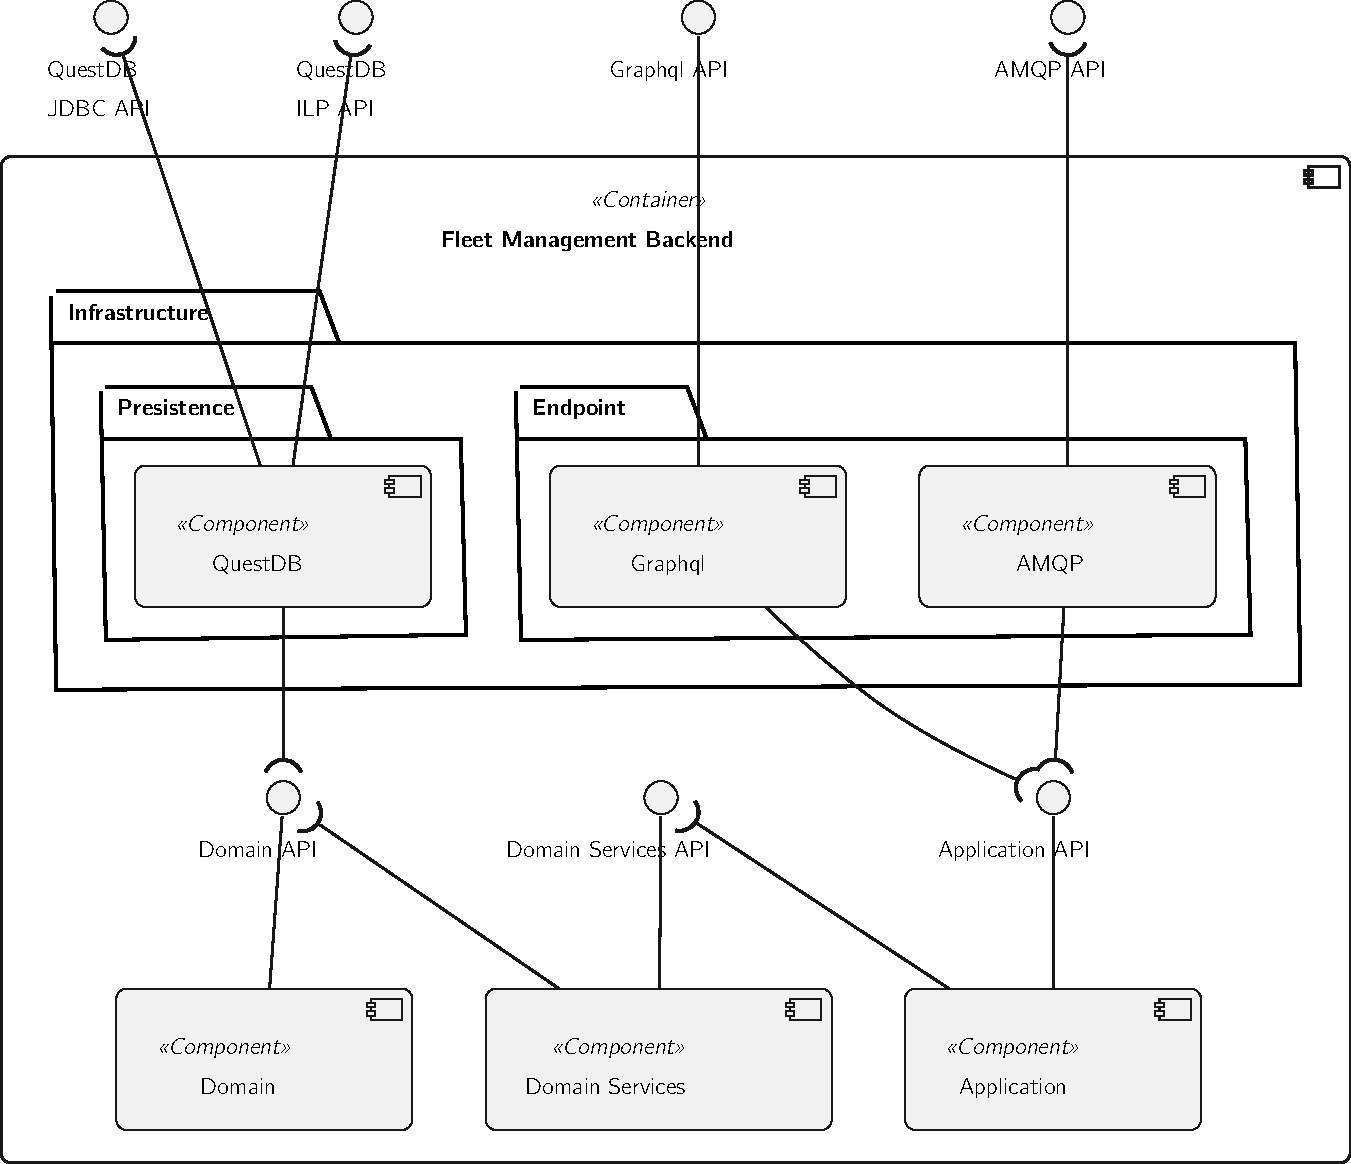
\includegraphics[page=1,width=0.8\columnwidth]{assets/diagrams/design/architectural/level3/logical/fleet-management-backend.pdf}
   \caption[Fleet Management Backend - Component Level - Logical View Diagram]{Fleet Management Backend - Component Level - Logical View Diagram}
   \label{fig:AppendixC2:fleet}
\end{figure}

\begin{figure}[H]
   \centering
   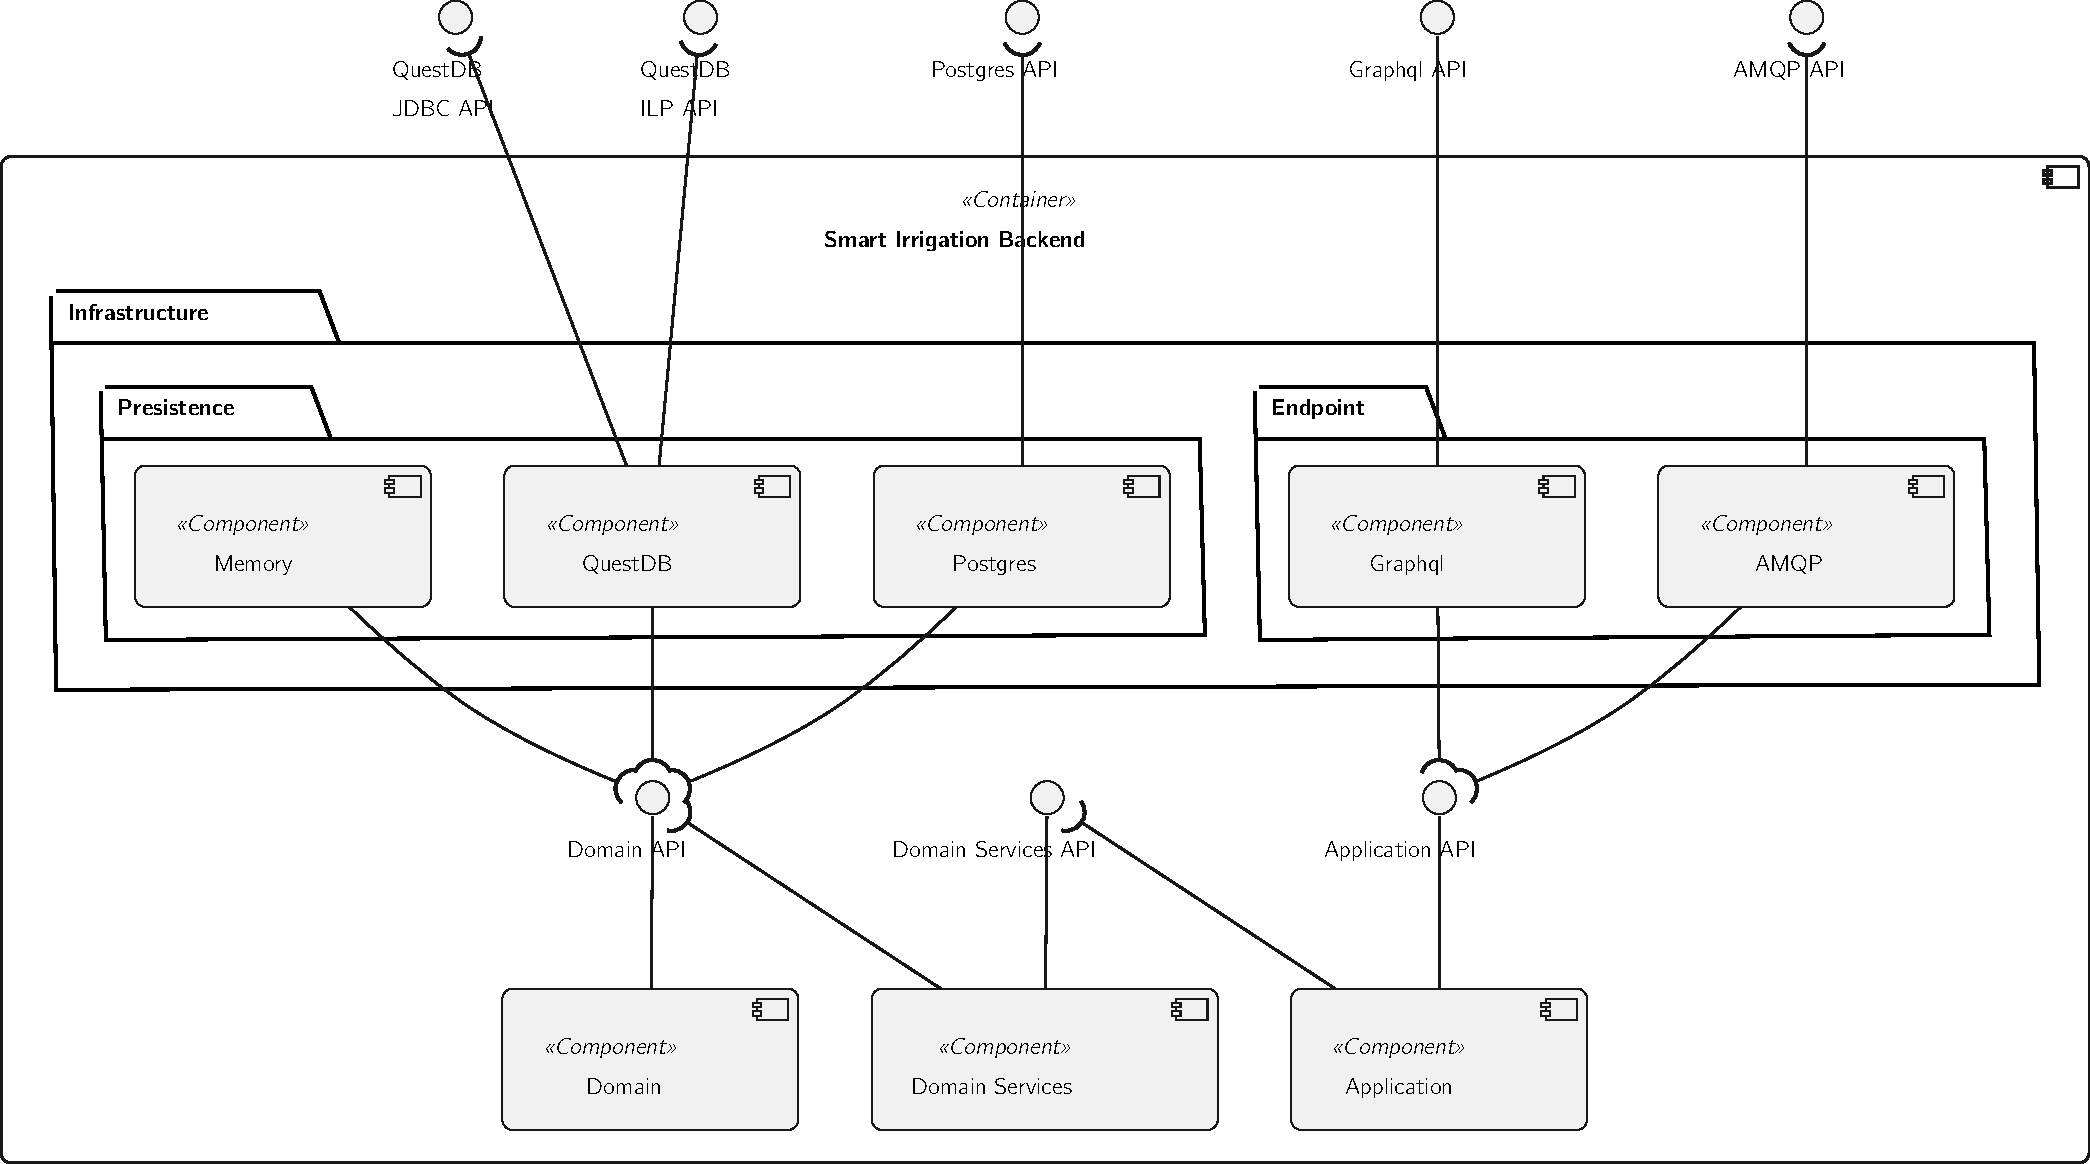
\includegraphics[page=1,width=\columnwidth]{assets/diagrams/design/architectural/level3/logical/smart-irrigation-backend.pdf}
   \caption[Smart Irrigation Backend - Component Level - Logical View Diagram]{Smart Irrigation Backend - Component Level - Logical View Diagram}
   \label{fig:AppendixC2:irrig}
\end{figure}

\begin{figure}[H]
   \centering
   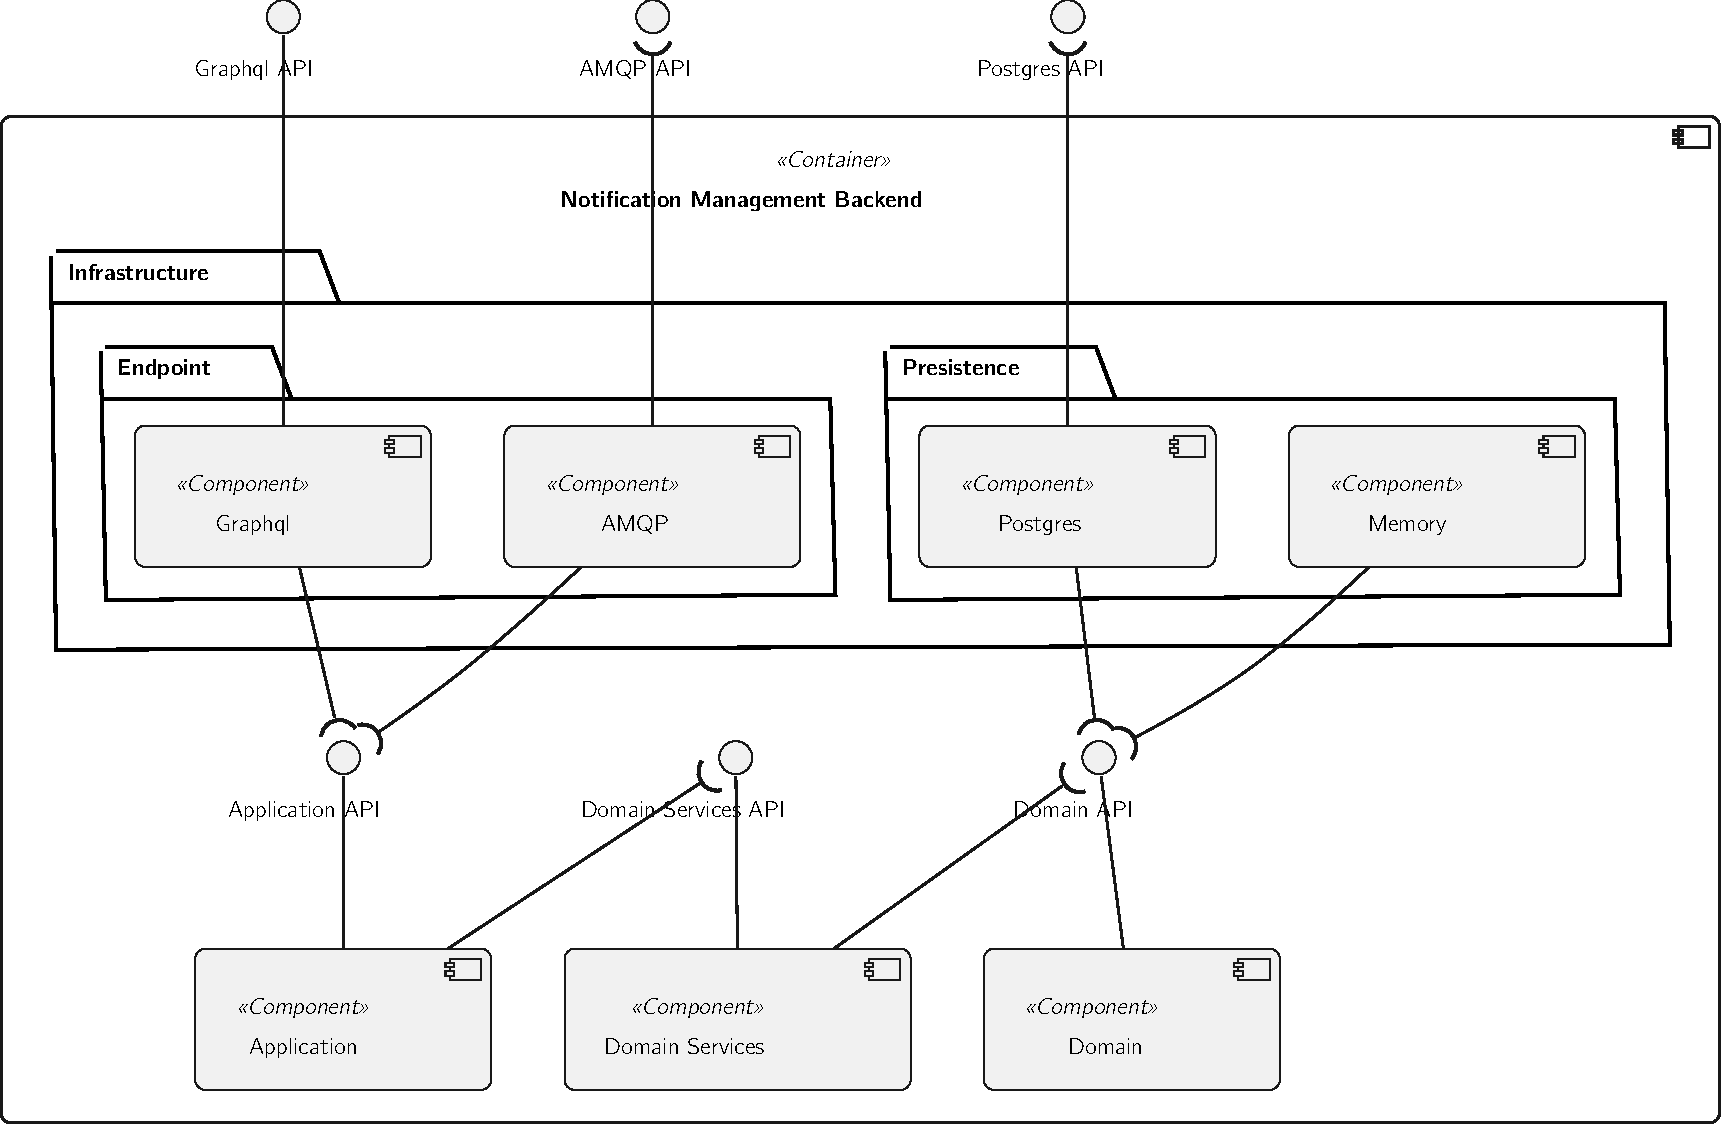
\includegraphics[page=1,width=\columnwidth]{assets/diagrams/design/architectural/level3/logical/notification-management-backend.pdf}
   \caption[Notification Management Backend - Component Level - Logical View Diagram]{Notification Management Backend - Component Level - Logical View Diagram}
   \label{fig:AppendixC2:noti}
\end{figure}

\begin{figure}[H]
   \centering
   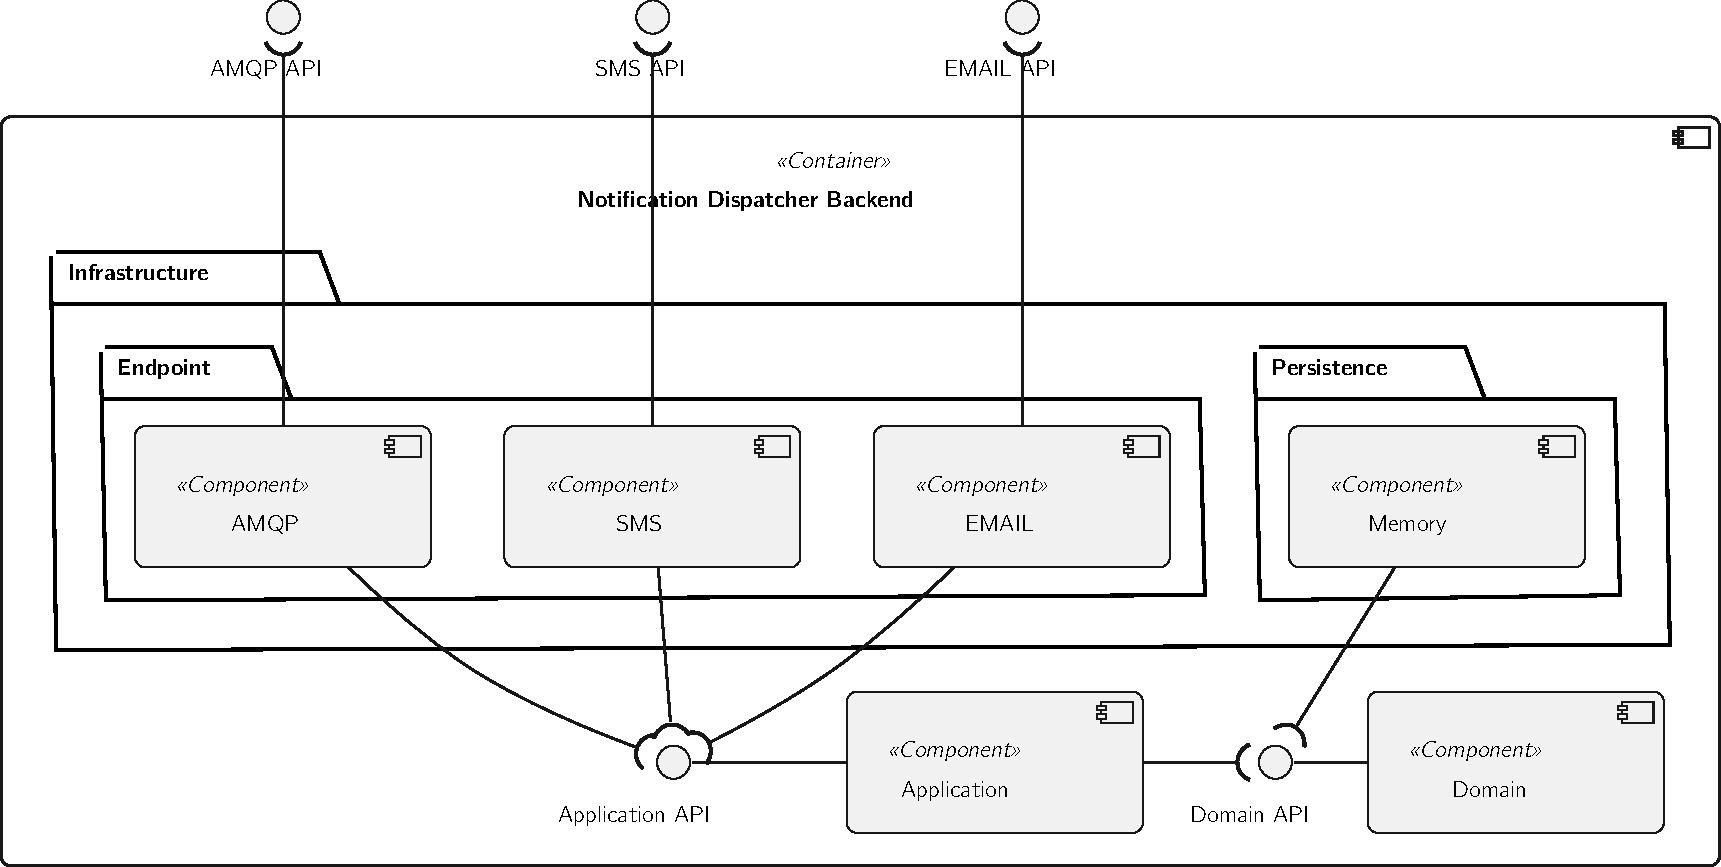
\includegraphics[page=1,width=\columnwidth]{assets/diagrams/design/architectural/level3/logical/notification-dispatcher-backend.pdf}
   \caption[Notification Dispatcher Backend - Component Level - Logical View Diagram]{Notification Dispatcher Backend - Component Level - Logical View Diagram}
   \label{fig:AppendixC2:notidispatcher}
\end{figure}
